\chapter{系统技术介绍}

\section{clang}
clang是LLVM项目中提供的一个编译器前端,服务于整个C语言家族。相比于GCC,clang提供了更迅捷的编译速度,更好的静态诊断信息
以及更灵活的架构。

除了作为编译器以外,clang还可以作为一个库来使用,开发者不必下载整个程序,可以选择库中自己所需要的工具,只使用一部分的编译器的功能,
例如源代码的生成和分析,本系统便利用来clang来获取c++源文件的AST。
\section{libclang}
考虑到clang本身是用c++语言编写的,故所有API全是c++形式的,但是c++接口本身具有版本更新带来的不稳定性以及c++
语言特性产生的复杂性,LLVM官方在介绍中并不推荐普通开发者使用clang的c++接口。

官方更加推荐的是其提供的c语言接口,其具有操作简单,运行稳定的优点。但是c语言本身缺少高级的抽象,开发难度大,
本系统采用了基于这套c语言接口的python binding,它在使用上与c语言接口是基本一致,环境配置也比c++更简单,
唯一的缺点是无法像c++一样获取完整的源程序AST,并且相比c++也缺少了一部分更细节层面的API,所以在某些情况下,只能自己手动分析。
\section{自动机}
自动机是计算机科学中一种常见的抽象模型,它可以识别一串符合输入规范的序列,并判断接受或者拒绝它。通常情况下,自动机由一个状态合集,一个可接收的字符合集以及一组状态转移函数组成。
状态代表自动机在运行期间的某一种运行状态,不同的输入字符排列组合成自动机接收的序列,状态转移函数描述了状态之间的转移。自动机可以在不同的状态之间转换,并根据输入符号执行相应的动作。
\subsection{确定有限状态自动机}
确定有限状态自动机(DFA)是一种特殊类型的自动机。
在DFA中,对于给定的输入符号和当前状态,仅存在唯一的可能的下一个状态。
DFA 是一种状态转移图,其中每个状态都与一个输入符号相关联,并确定了进入下一个状态的路径。
它使用确定性转移函数来处理输入,并可以准确地确定接受或拒绝输入序列。
\subsection{非确定有限状态自动机}
非确定有限状态自动机(NFA)是另一种类型的自动机。
与DFA不同,NFA允许在给定的输入符号和状态下存在多个下一个状态。
这意味着在NFA中,给定一个输入符号和当前状态,可以有多个选择进行状态转移。
NFA使用非确定性转移函数来处理输入的序列,也存在空边,并且无法确定唯一的状态转移路径。

本系统中,我们根据生成的CFG首先生成的只是相应的NFA,但是要想准确定位错误,能够将某一个状态具体对应到代码的某一段,我们还需要将NFA转换成
DFA,对于这一转换,本系统采用的是子集构造法。
\subsection{子集构造法}
子集构造法(Subset Construction Method)是一种将非确定有限状态自动机(NFA)转换为等价的确定有限状态自动机(DFA)的算法。
该算法的基本思想是根据NFA的状态集合构造DFA的状态集合,并在状态转移函数中处理相应的转移。

以下是子集构造法的大体步骤:
\begin{enumerate}
	\item  初始状态:
 从NFA的初始状态开始,构造DFA的初始状态,即将初始状态作为DFA的初始状态。
    \item  状态转移:
对于每个DFA状态和每个输入符号,找到对应的NFA状态集合。
对于该输入符号,将NFA状态集合进行ε-闭包处理,即找到所有通过ε(空转移)可以到达的状态。
将得到的ε-闭包状态集合作为DFA状态的转移目标,并根据输入符号找到相应的转移。
    \item  状态集合构建:
对于每个新构造的DFA状态,重复第二步骤,直到没有新的状态可以构造。
    \item  判断接受状态:
根据NFA的接受状态集合来判断DFA的接受状态。
如果DFA的状态集合中包含任何一个NFA的接受状态,则将该DFA状态标记为接受状态。
\end{enumerate}
通过使用子集构造法,可以将NFA转换为具有确定性的DFA。


\section{抽象语法分析树}
抽象语法树(Abstract Syntax Tree,AST)是一个用于代表程序代码层次结构的树状数据结构。许多编译器,解释器以及静态分析工具都是以此为
开发基础。AST通过将代码语法拆解成了抽象的语法树结构,提供了一种以层次化,结构化理解和处理代码的方式。代码提示,格式化,debug工具,或者自动生成序列化代码等等,这些功能的开发都需要语法树里面的信息。
AST将代码中的各个元素(如表达式Expression,语句Statement,声明Declaration等)转化为语法树中的节点,而节点之间通过父子关系建立连接。
通常情况下,AST的根节点表示整个代码文件,然后每个语法结构(如函数、循环、条件语句等)都成为根节点的子节点。子节点可以继续有自己的子节点,以此类推,形成一个树状结构。

\begin{figure}[htbp]
	\centering
	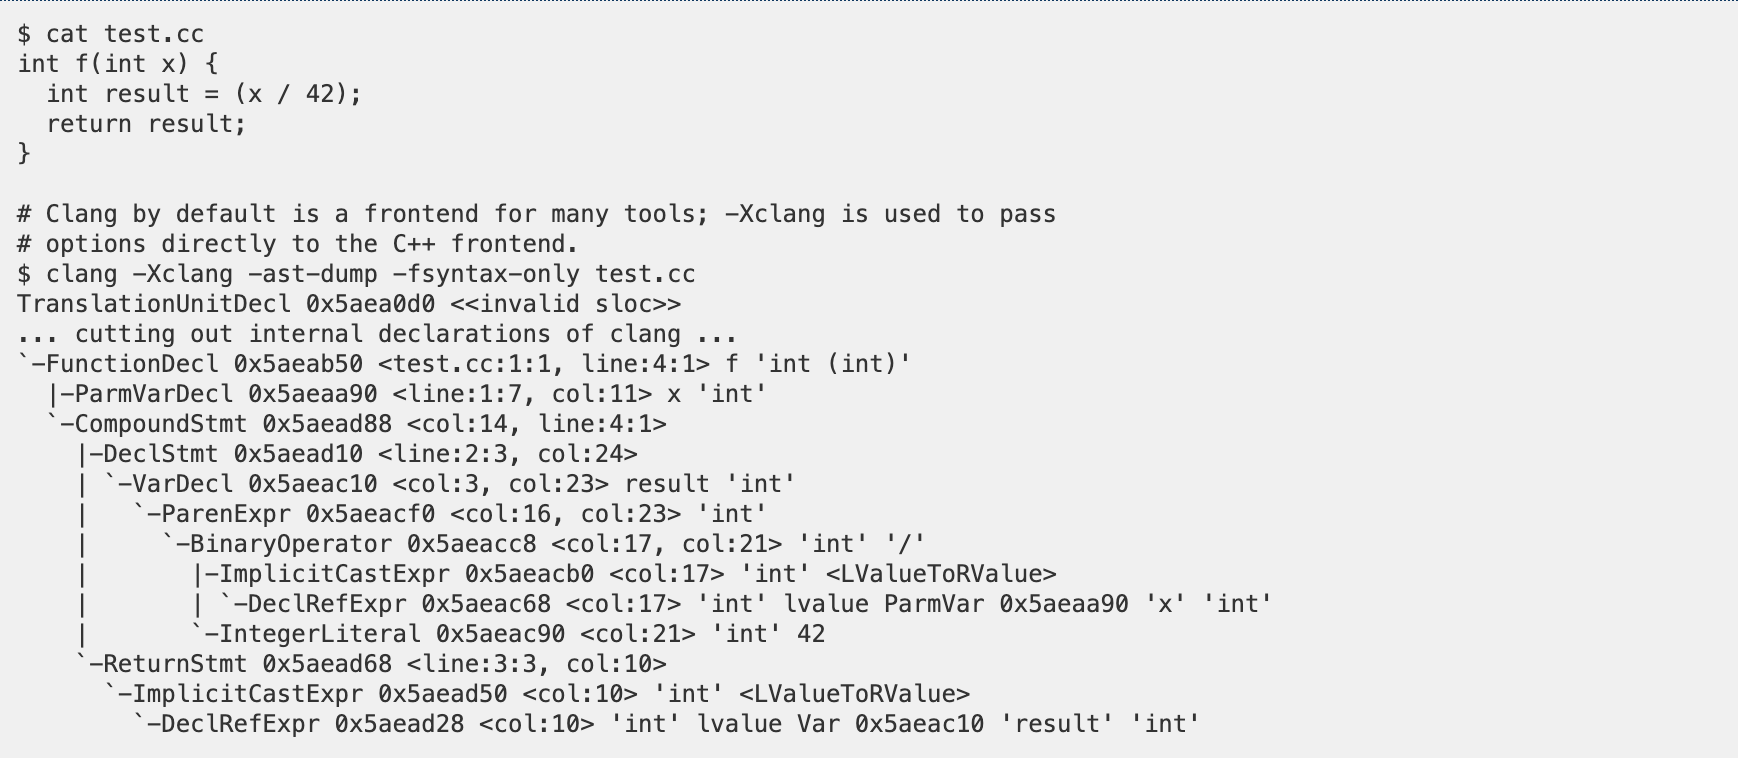
\includegraphics[width=1\textwidth]{pictures/clang-AST.png}
	\caption{clang-AST}
	\label{fig:my_label}
\end{figure}


在clang生成的ast中,其根节点是TranslationUnitDecl,代表了一个c++源文件,我们可以从此开始遍历整个AST树,也可以获取已解析的的标识符表。
clang的AST节点并没有一个共同的“NODE”基类,大部分AST节点派生自 Type、 Decl、 DeclContext 或Stmt,还有一些节点属于自己的特定结构。
因此,要遍历完整的AST,需要从TranslationUnitDecl开始,然后递归地遍历从该节点可以到达的所有内容,并针对每种特定节点类型对这一信息进行编码。该算法被编码在一个RecursiveASTVisitor中。
值得庆幸的是,对于libclang而言,相应的api已经帮我们处理好了这些复杂的类型,我们只需要简单地把它们统一处理即可。


\section{程序控制流图}
程序控制流图程序控制流图(Program Control Flow Graph)是一种用于表示程序执行流程的图形结构。
它描述了程序中不同语句之间的控制流结构。
程序控制流图有助于可视化和分析程序的结构,并在软件工程中广泛应用于代码分析、特别是数据流分析相关的技术。

一个程序控制流图由以下几个基本元素组成:
\begin{itemize}
	\item 基本块(Basic Block):基本块是程序控制流图的基本单元,它是一组语句的顺序执行序列。基本块内部没有分支和跳转语句,只有一个进入点和一个退出点。基本块可以包含多行代码,但通常被简化为单个语句。
    \item 控制边(Control Edge):控制边用于表示程序控制的转移关系。它连接了控制流图中的不同基本块,指示程序的执行流从一个基本块转移到另一个基本块。控制边也可以表示条件分支、循环结构和其他控制转移。
    \item 进入点(Entry Point):进入点是控制流图中的起始点,它标识程序的入口,表示程序开始执行的位置。
    \item 退出点(Exit Point):退出点是控制流图中的终止点,它标识程序的出口,表示程序结束执行的位置。
\end{itemize}
值得注意的是,在本系统中,我们关注的主要是由日志函数,所以并不需要真正的按照基本块生成CFG,而是将一条语句作为程序控制流图中的基本块,这有助于简化CFG的整体结构。

